\documentclass[]{beamer}
\usepackage[utf8]{inputenc}
\usepackage{xeCJK}
\usepackage{graphicx}
\usepackage{subfigure}
\usepackage{mathtools}
\usepackage{utopia} %font utopia imported
\usetheme{CambridgeUS}
\usecolortheme{dolphin}
\usefonttheme{professionalfonts}
\usepackage{natbib}
\usepackage{hyperref}
\usepackage{fontspec}
\usepackage{setspace}
\usepackage{float}
\usepackage{extarrows}
% \usepackage{enumitem}

\setCJKmainfont{SourceHanSansSC-Regular.otf}[Path=../, BoldFont=bold.otf]

\setbeamerfont{title}{size=\Large}
\setbeamerfont{subtitle}{size=\small}
\setbeamerfont{date}{size=\small}
\setbeamerfont{institute}{size=\small}

\setstretch{1.3}
% \setlength{\parindent}{2em}
% \setlength{\parskip}{0pt}

% \setlist[itemize]{leftmargin=2em}

% ↓↓↓ Modify this ↓↓↓
\title{高等数学I\quad 习题课07}
\subtitle{等价无穷小,函数的连续性}
\date[2025.10.30]{2025.10.30}
% ↑↑↑ Modify this ↑↑↑

\author[上海科技大学]{}
\institute[]{上海科技大学}

\begin{document}

\begin{frame}
    \vspace{15pt}
    \titlepage
\end{frame}

% \begin{frame}{Quiz}
%     \[
%     \text{\Huge 18:00 - 18:30}
%     \]
% \end{frame}

\begin{frame}{习题课06 反馈}
    \begin{columns}
        % 左栏:文字
        \begin{column}{0.5\textwidth}
            \begin{figure}[H]
                \centering
                
\includegraphics[width=1.0\linewidth]{fb1.png}
                \caption{课程质量}
            \end{figure}
        \end{column}

        \begin{column}{0.5\textwidth}
            \begin{figure}[H]
                \centering
                
\includegraphics[width=1.0\linewidth]{fb2.png}
                \caption{课堂氛围}
            \end{figure}
        \end{column}
    \end{columns}
\end{frame}

\begin{frame}{Reminder}
    \begin{itemize}
        \item 在完全了解定理背后的原理之前,不要轻易使用这些定理\\(非常容易出错)
        \item HW3,HW4大量出现洛必达,导数\dots
        \item 初等分析方法的练习对于日后进行复杂问题的分析是非常有必要的\\ (有利于建立数学直观)
        \item 你可以:
        \begin{itemize}
            \item 先使用高阶方法,得到问题的答案
            \item 再根据高阶方法的求解过程,思考如何使用初等方法解决问题
        \end{itemize}
    \end{itemize}
\end{frame}

\begin{frame}{目录}
    \tableofcontents
\end{frame}

\AtBeginSection[ ]
{
\begin{frame}{目录}
    \tableofcontents[currentsection]
\end{frame}
}

\section{函数极限}

\begin{frame}{23 Fall, ch.2 Quiz (Revisited)}
    用$\varepsilon-\delta$语言证明:
    \[
    \lim_{x\rightarrow2}x^2=4
    \]
\end{frame}

\begin{frame}{思路}
    \begin{itemize}
        \item 目标:找到$\delta$,使得对于所有$0<|x-a|<\delta$,都有$|f(x)-A|<\varepsilon$
        \item 不可避免地,需要凑出$|x-a|$以将$|f(x)-A|<\varepsilon$变为$g(x)\delta<\varepsilon$
        \item 善用放缩,避免硬解
    \end{itemize}
\end{frame}

\begin{frame}{两个重要极限}
    \[
    \lim_{x\rightarrow0}\frac{\sin x}{x}=1\qquad\lim_{x\rightarrow\infty}(1+\frac1x)^x=e
    \]
    怎么用?
\end{frame}

\begin{frame}{用法}
    \begin{itemize}
        \item $\displaystyle\lim_{x\rightarrow0}\frac{\sin x}{x}=1$:用于三角函数向线性函数的拟合\\ \vspace{5pt}
        (今日内容:泰勒展开的几何理解)
        \item $\displaystyle\lim_{x\rightarrow\infty}(1+\frac1x)^x=e$:用于$(1+0)^\infty$形极限,且$0$项与$\infty$项互为倒数
    \end{itemize}
\end{frame}


\begin{frame}{典型错误}
    求
    \[
    \lim_{x\rightarrow\infty}\frac{(1+\frac1x)^{x^2}}{e^x}
    \]
\end{frame}

\begin{frame}{投票}

\end{frame}

\begin{frame}{注意事项}
    \begin{itemize}
        \item 对某个表达式取极限时,该表达式内被取极限的变量的趋近于同一个值
    \end{itemize}
\end{frame}

\section{无穷小}

\begin{frame}{定义}
    若$x\rightarrow a$时,$f(x)\rightarrow 0, g(x)\rightarrow 0$,考虑$\displaystyle\lim_{x\rightarrow a}\frac{f(x)}{g(x)}=l\in\mathbb R$:
    \begin{itemize}
        \item $l=0\Leftrightarrow$\\$x\rightarrow a\text{ 时,} f(x)$是比$g(x)$高阶的无穷小,记作$f(x)=o(g(x))$
        \item $l\ne0\Leftrightarrow$\\$x\rightarrow a\text{ 时,} f(x)$是与$g(x)$同阶的无穷小,记作$f(x)=O(g(x))$.\\
        若$l=1$则称$x\rightarrow a\text{ 时,}f(x)$与$g(x)$是等价无穷小,$f(x)\sim g(x)$.
    \end{itemize}
    \vspace{5pt}
    我们将在第四章更详细地讲解等价无穷小的概念。
\end{frame}

\begin{frame}{几何理解}
    $y=x,x^2,x^3,x^4$在$x=0$附近的图像:
    \begin{figure}[H]
        \centering
        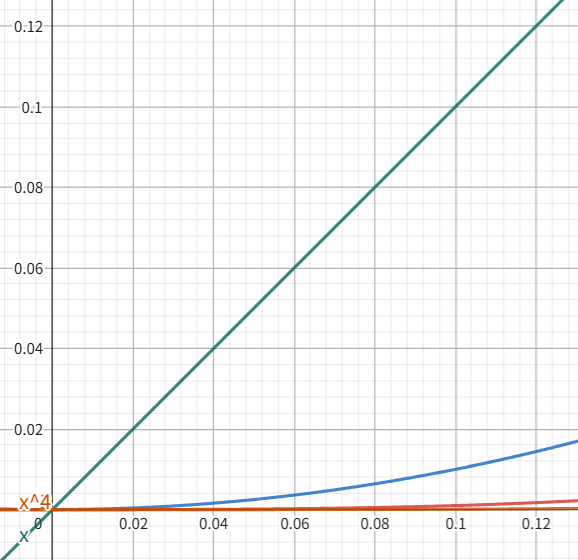
\includegraphics[width=0.45\linewidth]{infi.png}
    \end{figure}
    \textbf{无穷小之间的大小亦有差别}
\end{frame}

\begin{frame}{定义}
    若$\displaystyle\lim_{x\rightarrow a}f(x)=0,$且存在常数$c\ne0,k>0,$使得
    \[
    \lim_{x\rightarrow a}\frac{f(x)}{(x-a)^k}=c,
    \]
    则称$x\rightarrow a$时,$f(x)$是\textbf{标准无穷小}$x-a$的$k$阶无穷小,简称$f(x)$是$k$阶无穷小,$c(x-a)^k$是$f(x)$的主部
\end{frame}

\begin{frame}{泰勒定理1}
教材定理4.9

设函数$f(x)$在点$x_0$的邻域内有定义,且在$x_0$处有$n$阶导数,那么
\[
f(x)=f(x_0)+f'(x_0)(x-x_0)+\cdots+\frac{f^{(n)}(x_0)}{n!}(x-x_0)^n+o((x-x_0)^n)
\]    
\end{frame}

\begin{frame}{$\cos(x)$在$0$处的多项式估计}
    \begin{itemize}
        \item 尝试使用$g(x)=c_0+c_1x+c_2x^2+c_3x^3+\cdots$拟合函数$\cos(x)$
        \item 基本想法:$0$处的函数值至少要相等$\Rightarrow g(0)=1\Rightarrow c_0=1$
        \item 切线斜率相等$\Rightarrow g'(x)|_{x=0}=\cos'(x)|_{x=0} \Rightarrow c_1 = 0$
        \item 继续?
    \end{itemize}
\end{frame}

\begin{frame}{$\cos(x)$在$0$处的多项式估计}
    \begin{itemize}
        \item 尝试使用$g(x)=c_0+c_1x+c_2x^2+c_3x^3+\cdots$拟合函数$\cos(x)$
        \item $c_0=1,c_1=0$
        \item 对$\cos(x)$的切线斜率在$x=0$附近的微小变动进行拟合
        \\ $\Rightarrow \cos''(x)|_{x=0} = g''(x)|_{x=0} \Rightarrow c_2 = -\frac12$ 
        \item $\cos(x) \approx 1 + 0x - \frac12x^2$
    \end{itemize}
\end{frame}

\begin{frame}{常用无穷小}
    \[
    \begin{array}{lll}
        \sin x\sim x\qquad&\tan x\sim x\qquad& 1-\cos x\sim\frac12 x^2\\
        \ln(1+x)\sim x\qquad&e^x-1\sim x\qquad&(1+x)^\alpha -1 \sim \alpha x\\
        \arcsin x\sim x\qquad&\arctan x\sim x
    \end{array}
    \]
    
\end{frame}


\begin{frame}{使用方法}
    \begin{itemize}
        \item 乘除:等价无穷小可以替换
        \item 加减:等价无穷小\textbf{有条件地}替换
    \end{itemize}
\end{frame}

\begin{frame}{简例}
    $f(x)=x+2x^2,g(x)=x-3x^2$,计算
    \[
    \lim_{x\rightarrow 0}\frac{f(x)-g(x)}{x^2}
    \]
\end{frame}

\begin{frame}{注意事项}
    \begin{itemize}
        \item 乘除运算不会导致无穷小的主部消失;
        \item 加减运算可能会导致无穷小主部恰好抵消,则此时剩余的更高阶无穷小\textbf{不可忽略}.
    \end{itemize}
\end{frame}

\begin{frame}{例 (24Fall Midterm 7.)}
    设$\displaystyle\lim_{x\rightarrow0}\frac{\cos x - 1 + f(x)}{x^3}=1$,求$\displaystyle\lim_{x\rightarrow0}\frac{f(x)}{\sin^2x}$
\end{frame}

\section{函数的连续性}

\begin{frame}{思考}
    如果一个函数连续,那么它应该满足什么性质?
    \begin{itemize}
        \item 当自变量的值变动很小的时候?
        \item 函数值也应当只变动了一点
    \end{itemize}
\end{frame}

\begin{frame}{数学语言}
    \begin{itemize}
        \item 自变量的值变动很小:原本为$x_0$,变为$x_0+\delta(\delta>0)$\\ $\Rightarrow \text{对所有在区间}(x_0,x_0+\delta)$的值,都应有\dots
        \item 函数值只变动\textbf{很小一点}:
        \[
        \forall \varepsilon>0, |f(x_0+\delta)-f(x_0)|<\varepsilon\quad\Rightarrow\quad\lim_{x\rightarrow x_0^+}f(x)=f(x_0)
        \]
        \item 若将$\delta$的取值范围限制为$\mathbb R$,则得到$\displaystyle\lim_{x\rightarrow x_0}f(x)=f(x_0)$
    \end{itemize}
\end{frame}

\begin{frame}{定义}
    设函数$f$在点$x_0$的某邻域内有定义,若
    \[
    \lim_{x\rightarrow x_0}f(x)=f(x_0),
    \]
    则称函数$f(x)$在$x_0$处\textbf{连续},称$x_0$是$f(x)$的\textbf{连续点};否则称$f(x)$在$x_0$处\textbf{间断},称$x_0$是$f(x)$的\textbf{间断点}.

    \begin{itemize}
        \item 类似地,将$x\rightarrow x_0$修改为$x_0^+$或$x_0^-$时,我们分别得到右连续、左连续的定义。
        \item 因此,$\displaystyle\lim_{x\rightarrow x_0}f(x)=f(x_0) \quad\Leftrightarrow\quad \lim_{x\rightarrow x_0^-}f(x)=\lim_{x\rightarrow x_0^+}f(x)=f(x_0)$
    \end{itemize}
\end{frame}

\begin{frame}{例(课本习题2 补充题5)}
    设函数$f(x)$在$(0,+\infty)$上满足$f(2x)=f(x)$,且$\displaystyle\lim_{x\rightarrow+\infty}f(x)=A$(有限值),证明:
    \[
    f(x)\equiv A.
    \]
    
\end{frame}

\begin{frame}{例(课本习题2 补充题6)}
    设在$\mathbb R$上定义的函数$f(x)$满足:
    \[
    f(x+y)=f(x)+f(y)\qquad(x,y\in\mathbb R),
    \]
    且在$x=0$处连续.证明:$f(x)\in C(\mathbb R)$
\end{frame}

\begin{frame}{间断点}
    \begin{itemize}
        \item 第一类间断点:左、右极限都存在
        \begin{itemize}
            \item 左右极限相等:可去间断点,表现为从完整的函数图像上挖去了一个点
            \item 左右极限不相等:跳跃间断点,表现为函数图像上出现了不连续的函数值变化(且变化前后都为有限值)
        \end{itemize}
        \item 第二类间断点:左、右极限不都存在
        \begin{itemize}
            \item 其中之一为无穷:无穷间断点
            \item 极限都不为无穷,但极限也不存在:振荡间断点(典例:$\sin\frac1x$)
        \end{itemize}
    \end{itemize}
    学会求间断点的值、判断间断点的类型
\end{frame}

\begin{frame}{投票}
    函数$g(x)=x\sin\frac1x$在$x=0$处的间断点类型为?
    
    可去间断点
\end{frame}

\begin{frame}{连续函数的运算}
    给定两个在$x_0$处连续的函数$f(x),g(x)$,$c$是常数,则:
    \begin{itemize}
        \item $f(x)+g(x),f(x)-g(x),cf(x),f(x)\cdot g(x)$在$x_0$处连续
        \item 当$g(x)$在$x_0$处不为0,$\frac{f(x)}{g(x)}$在$x_0$处连续
    \end{itemize}
\end{frame}

\begin{frame}{复合函数的连续性}
    与复合函数的极限类似,设函数$\varphi(x)$在点$x_0$处连续,而函数$f(x)$在点$u_0=\varphi(x_0)$处连续,
    则复合函数$f\circ \varphi =f(\varphi(x))$在点$x_0$连续.
\end{frame}

% \section{作业}

% \begin{frame}{HW2.T13.1}
%     设数集$E$有上界,证明:数集$-E:=\{x|-x\in E\}$有下界,且$\sup E = -\inf(-E)$.
% \end{frame}

% \begin{frame}{HW2.T13.2}
%     对非空数集$A,B$,定义其和为$A+B:=\{a+b|a\in A,\ b\in B\}.$
%     证明:若$A,B$皆有上界,则$A+B$亦有上界,且$\sup(A+B)=\sup A+\sup B.$
% \end{frame}

% \begin{frame}{HW2.T13.3}
%     若数列$a_n$满足$a_n<qa_{n-1}$,其中$a_n>0,0<q<1$,试用定义证明$\lim\limits_{n\rightarrow\infty}a_n=0$.
% \end{frame}

% \begin{frame}{HW2.T13.4}
%     设有数列$\{a_n\}$和$\{b_n\}$,如果$\lim\limits_{n\rightarrow\infty}\frac{a_n}{b_n}=a(a\ne0)$且$\lim\limits_{n\rightarrow\infty}a_n=0$,
%     证明$\lim\limits_{n\rightarrow\infty}b_n=0.$
% \end{frame}

% \section*{}
% \begin{frame}{反馈问卷}
%     \begin{figure}[H]
%         \centering
%         
\includegraphics[width=0.5\linewidth]{qrcode.png}
%     \end{figure}
% \end{frame}


% -------------------------------------------------------
% \section*{}
% \begin{frame}
% \vspace{25pt}
% \[
% \text{\Huge Office Hour}
% \]
% \end{frame}

\end{document}